\documentclass{standalone}
\usepackage{tikz}
\usepackage{ctex,siunitx}
\usepackage{tkz-euclide}
\usepackage{amsmath}
\usetikzlibrary{patterns, calc}
\usetikzlibrary {decorations.pathmorphing, decorations.pathreplacing, decorations.shapes,}
\begin{document}
\small
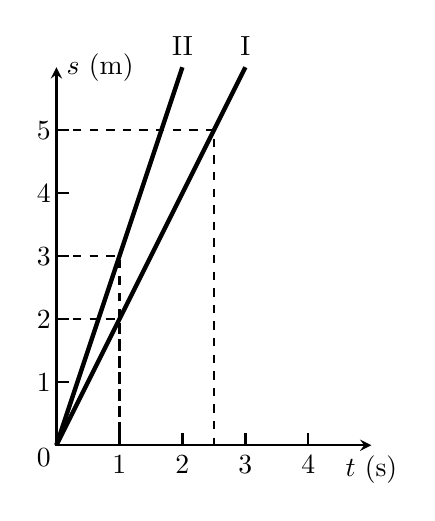
\begin{tikzpicture}[>=stealth, thick,scale=0.8]
  \draw [<->] (0,6) node[right]{$s$ (\unit{m})}--(0,0)--(5,0)node[below]{$t$ (\unit{s})};
  \foreach \x in {1,2,...,4}
  {
      \draw (\x,0)--(\x, 0.2);
      \draw (0,\x)--(0.2, \x);
  \node at (\x, -.3){$\x$};
  \node at (-.2,\x){$\x$};
  }
  \node at (-.2,-.2){0};
  \draw (0,5)--(0.2, 5);
  \node at (-.2,5){$5$};
  \draw[dashed] (0,2)--(1,2)--(1,0);
  \draw[dashed] (0,3)--(1,3)--(1,0);
  \draw[dashed] (0,5)--(2.5,5)--(2.5,0);
  \draw [ultra thick](0,0)--(3,6) node [above]{I};
  \draw [ultra thick](0,0)--(2,6) node [above]{II};
\end{tikzpicture}
\end{document}